\documentclass[12pt]{article}
\newif\ifanswer\answertrue%\answerfalse% comment out to show/hide answers
\usepackage{../preamble3}% preamble always after \newif\ifanswer
%\pagenumbering{gobble}
\title{Art Of Problem Solving - AMC 10 \\ August 7, 2021}
\author{Patrick \& James Toche}
\date{Revised:~\today}

\begin{document}
\maketitle
\begin{minipage}{\textwidth}
\begin{abstract}\setlength{\parindent}{0pt}%
Notes on the AMC-10 Course by Art Of Problem Solving (AOPS).
Copyright restrictions may apply. Written for personal use. 
Please report typos and errors over at \url{https://github.com/ptoche/Math/tree/master/aops}. 
\end{abstract}
\end{minipage}

\thispagestyle{empty}
\clearpage


%%%%%%%%%%%%%%%%%%%%%%%%%%%%%%%%%%%%%%%%%%%%%%%%%%%%%%%%%%%%%%%%%%%%%%%%
\subsection*{1.}

\nopagebreak

Henry's Hamburger Heaven offers its hamburgers with the following condiments: ketchup, mustard, mayonnaise, tomato, lettuce, pickles, cheese, and onions. A customer can choose one, two, or three meat patties, and any collection of condiments. How many different kinds of hamburgers can be ordered?

\fbox{(A) $24$ \quad (B) $256$ \quad (C) $768$ \quad (D) $40,320$ \quad (E) $120,960$}

\begin{answer}
There are $8$ choices of condiments which may be combined in any way. Thus, for each condiment, it is either selected $1$ or not $0$ --- two choices. The total number of ways is therefore $2^8=256$. There are $3$ choices for the meat, and therefore $256\times3=768$ different kinds of orders. 
\begin{empheq}[box={\mathbox[colback=white]}]{equation*}
    768
\end{empheq} 
\end{answer}
%%%%%%%%%%%%%%%%%%%%%%%%%%%%%%%%%%%%%%%%%%%%%%%%%%%%%%%%%%%%%%%%%%%%%%%%

\iftoggle{showAnswers}{\newpage}

%%%%%%%%%%%%%%%%%%%%%%%%%%%%%%%%%%%%%%%%%%%%%%%%%%%%%%%%%%%%%%%%%%%%%%%%
\subsection*{2.}

\nopagebreak

At an inter-species dance party, each cat danced with exactly three dogs and each dog danced with exactly two cats. No one danced with anyone of their own species, and twelve cats attended the party. How many dogs attended the party?

\fbox{(A) $8$ \quad (B) $12$ \quad (C) $16$ \quad (D) $18$ \quad (E) $24$}


\begin{answer}
Let $c$ denote the number of cats and $d$ the number of dogs. The total number of pairs is:
\begin{align*}
3 c & = 2d \\
\text{where}~
  c & = 12 \\
\quad\Rightarrow\quad
         d & = \frac{3 \times 12}{2} = 18
\end{align*}
\begin{empheq}[box={\mathbox[colback=white]}]{equation*}
    18 ~\text{dogs}
\end{empheq} 
\end{answer}
%%%%%%%%%%%%%%%%%%%%%%%%%%%%%%%%%%%%%%%%%%%%%%%%%%%%%%%%%%%%%%%%%%%%%%%%

\iftoggle{showAnswers}{\newpage}

%%%%%%%%%%%%%%%%%%%%%%%%%%%%%%%%%%%%%%%%%%%%%%%%%%%%%%%%%%%%%%%%%%%%%%%%
\subsection*{3.}

\nopagebreak

A restaurant offers three desserts, and exactly twice as many appetizers as main courses. A dinner consists of an appetizer, a main course, and a dessert. What is the least number of main courses that the restaurant should offer so that a customer could have a different dinner each night in the year 2003?

\fbox{(A) $4$ \quad (B) $5$ \quad (C) $6$ \quad (D) $7$ \quad (E) $8$}


\begin{answer}
There are $365$ dinners in the year. Let $n$ denote the number of main courses to be offered during the year. We want to be able to select $1$ dessert from $3$, together with $1$ appetizers from $2n$, and $1$ main course from $n$, so that
\begin{align*}
\binom{3}{1} \cdot \binom{2n}{1} \cdot \binom{n}{1} 
  & \geq 365 \\
3 \cdot 2n \cdot n   
  & \geq 365 \\
n & \geq \sqrt{\frac{365}{6}} \approx 7.8 
\end{align*}
Thus, $8$ main courses are required at least. 
\begin{empheq}[box={\mathbox[colback=white]}]{equation*}
    8
\end{empheq} 
\end{answer}
%%%%%%%%%%%%%%%%%%%%%%%%%%%%%%%%%%%%%%%%%%%%%%%%%%%%%%%%%%%%%%%%%%%%%%%%

\iftoggle{showAnswers}{\newpage}

%%%%%%%%%%%%%%%%%%%%%%%%%%%%%%%%%%%%%%%%%%%%%%%%%%%%%%%%%%%%%%%%%%%%%%%%
\subsection*{4.}

\nopagebreak

A license plate in a certain state consists of 4 digits, not necessarily distinct, and 2 letters, also not necessarily distinct. These six characters may appear in any order, except that the two letters must appear next to each other. How many distinct license plates are possible?

\fbox{(A) $10^{4}\cdot26^{2}$ \quad (B) $10^{3}\cdot26^{3}$ \quad (C) $5\cdot10^{4}\cdot26^{2}$ \quad (D) $10^{2}\cdot26^{4}$ \quad (E) $5 \cdot 10^{3}\cdot26^{3}$}

\begin{answer}
There are $10^4$ possible combinations of digits and $26^2$ possible combinations of letters. Since the letters must appear next to each other, there are $5$ possibilities: they could appear in position $(1,2)$, $(2,3)$, $(3,4)$, $(4,5)$, $(5,6)$. The answer is therefore
\begin{empheq}[box={\mathbox[colback=white]}]{equation*}
    5 \cdot 10^4 \cdot 26^2
\end{empheq} 
\end{answer}
%%%%%%%%%%%%%%%%%%%%%%%%%%%%%%%%%%%%%%%%%%%%%%%%%%%%%%%%%%%%%%%%%%%%%%%%

\iftoggle{showAnswers}{\newpage}
  
%%%%%%%%%%%%%%%%%%%%%%%%%%%%%%%%%%%%%%%%%%%%%%%%%%%%%%%%%%%%%%%%%%%%%%%%
\subsection*{5.}

\nopagebreak

A set of 25 square blocks is arranged into a $5 \times 5$ square. How many different combinations of 3 blocks can be selected from that set so that no two are in the same row or column?

\fbox{(A) $100$ \quad (B) $125$ \quad (C) $600$ \quad (D) $2300$ \quad (E) $3600$}

\begin{answer}
Consider placing the blocks sequentially. There are $25$ choices for the first block. After the first block has been placed, that row and column are no longer available, that leaves $25-9=16$ blocks to choose from. After that, $16-7=9$ blocks to choose from, so the total number of ways to position $3$ blocks on $25$ squares is:
\begin{align*}
25 \cdot 16 \cdot 9 = 3600
\end{align*}
But since there is no way to distinguish these blocks, we are overcounting. We have overcounted the first square by a factor of $3$ and the second square by a factor of $2$. The required correction is therefore $3!$.
\begin{align*}
\frac{25 \cdot 16 \cdot 9}{3!} = \frac{3600}{6} = 600
\end{align*}
\begin{empheq}[box={\mathbox[colback=white]}]{equation*}
    600
\end{empheq} 

In this example, it is easy to keep track of the available squares. In general, for large grids, it is useful to have a systematic approach. Consider an $m$ by $n$ grid. The figure shows one block (blue) and the squares that subsequently become unavailable (red). The precise position of the block is irrelevant, as can be seen from several examples.
\begin{center}
  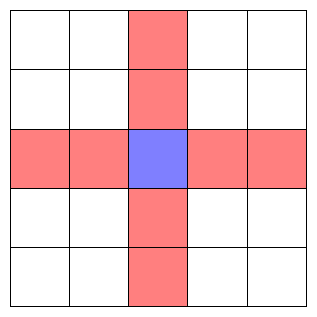
\includegraphics[height=2cm,page=1]{2021-08-07-figure-05}\hspace{20pt}
  \includegraphics[height=2cm,page=2]{2021-08-07-figure-05}
\end{center}
After the first block has been positioned, the problem is equivalent to one with an $m-1$ by $n-1$ grid. And the process goes on. 
\begin{center}
  \includegraphics[height=2cm,page=2]{2021-08-07-figure-05}\hspace{20pt}
  \includegraphics[height=2cm,page=3]{2021-08-07-figure-05}\hspace{20pt}
  \includegraphics[height=2cm,page=4]{2021-08-07-figure-05}
\end{center}
Thus the total number of ways to position $b$ blocks on an $mn$ grid is:
\begin{align*}
\frac{mn \cdot (m-1)(n-1) \cdot \ldots \cdot (m-b+1) (n-b+1)}{b!}
\end{align*}
\end{answer}
%%%%%%%%%%%%%%%%%%%%%%%%%%%%%%%%%%%%%%%%%%%%%%%%%%%%%%%%%%%%%%%%%%%%%%%%

\iftoggle{showAnswers}{\newpage}

%%%%%%%%%%%%%%%%%%%%%%%%%%%%%%%%%%%%%%%%%%%%%%%%%%%%%%%%%%%%%%%%%%%%%%%%
\subsection*{6.}

\nopagebreak

Pat is to select six cookies from a tray containing only chocolate chip, oatmeal, and peanut butter cookies. There are at least six of each of these three kinds of cookies on the tray. How many different assortments of six cookies can be selected?

\fbox{(A) $22$ \quad (B) $25$ \quad (C) $27$ \quad (D) $28$ \quad (E) $729$}

\begin{answer}
There are enough cookies to select $6$ of one (and any) kind only. There are $3$ kinds of cookies. The total number of cookies is unknown and clearly unimportant. The number of assortments of one kind only is $3$. To divide the cookies into three groups, we need two dividers. Applying the stars and bars formula, we get
\begin{align*}
\binom{6+2}{2} = \frac{8!}{6!2!} = \frac{8 \cdot 7}{2} = 28
\end{align*}
\begin{empheq}[box={\mathbox[colback=white]}]{equation*}
    28
\end{empheq} 
\end{answer}
%%%%%%%%%%%%%%%%%%%%%%%%%%%%%%%%%%%%%%%%%%%%%%%%%%%%%%%%%%%%%%%%%%%%%%%%

\iftoggle{showAnswers}{\newpage}

%%%%%%%%%%%%%%%%%%%%%%%%%%%%%%%%%%%%%%%%%%%%%%%%%%%%%%%%%%%%%%%%%%%%%%%%
\subsection*{7.}

\nopagebreak

Seven distinct pieces of candy are to be distributed among three bags. The red bag and the blue bag must each receive at least one piece of candy; the white bag may remain empty. How many arrangements are possible?

\fbox{(A) $1930$ \quad (B) $1931$ \quad (C) $1932$ \quad (D) $1933$ \quad (E) $1934$}

\begin{answer}
There are $3^{7}$ ways to place $7$ pieces into $3$ bags, neglecting restrictions. The first restriction is that the red bag cannot be empty: there are $2^{7}$ ways to place $7$ candies into $2$ bags only, leaving the red bag empty, so we must subtract these cases. Likewise for the blue bag. However, the case where both the red and blue bags are empty is included in both counts. Putting it together,
\begin{align*}
3^{7} - 2 \cdot 2^{7} + 1
= 1932
\end{align*}
\begin{empheq}[box={\mathbox[colback=white]}]{equation*}
    x
\end{empheq} 
\end{answer}
%%%%%%%%%%%%%%%%%%%%%%%%%%%%%%%%%%%%%%%%%%%%%%%%%%%%%%%%%%%%%%%%%%%%%%%%

\iftoggle{showAnswers}{\newpage}

%%%%%%%%%%%%%%%%%%%%%%%%%%%%%%%%%%%%%%%%%%%%%%%%%%%%%%%%%%%%%%%%%%%%%%%%
\subsection*{8.}

\nopagebreak

Two subsets of the set $S = \{a,b,c,d,e\}$ are to be chosen so that their union is $S$ and their intersection contains exactly two elements. In how many ways can this be done, assuming that the order in which the subsets are chosen does not matter?

\fbox{(A) $20$ \quad (B) $40$ \quad (C) $60$ \quad (D) $160$ \quad (E) $320$}

\begin{answer}
An example of two subsets that fit the criteria are $\{a,b,c,d,e\}$ and $\{a,b\}$. Another example is $\{a,b,c,d\}$ and $\{a,b,e\}$. Yet another example is $\{a,b,c,e\}$ and $\{a,b,d\}$. And lastly, $\{a,b,c\}$ and $\{a,b,d,e\}$. How many pairs of subsets have intersection $\{a,b\}$? We have enumerated $4$. This can be explained as follows. Since $a$ and $b$ must appear in both subsets and the other elements $c$, $d$, $e$ must appear exactly once in any of the subsets, that gives $2^{3}/2=4$ ways to split the $3$ elements two ways (we divide by two because identical subsets are indistinguishable). There are $\binom{5}{2}$ ways to select pairs from $5$ elements. 
\begin{align*}
4 \cdot \binom{5}{2}
= 4 \cdot \frac{5!}{2!3!} = 40
\end{align*}
\begin{empheq}[box={\mathbox[colback=white]}]{equation*}
    40
\end{empheq} 
\end{answer}
%%%%%%%%%%%%%%%%%%%%%%%%%%%%%%%%%%%%%%%%%%%%%%%%%%%%%%%%%%%%%%%%%%%%%%%%

\iftoggle{showAnswers}{\newpage}

%%%%%%%%%%%%%%%%%%%%%%%%%%%%%%%%%%%%%%%%%%%%%%%%%%%%%%%%%%%%%%%%%%%%%%%%
\subsection*{9.}

\nopagebreak

The entries in a $3 \times 3$ array include all the digits from 1 through 9, arranged so that the entries in every row and column are in increasing order. How many such arrays are there?

\fbox{(A) $18$ \quad (B) $24$ \quad (C) $36$ \quad (D) $42$ \quad (E) $60$}

\begin{answer}
One approach is to fill the grid with admissible numbers, subdividing cases into groups, and adding up the possibilities. The figure shows a graph. 
\begin{center}
  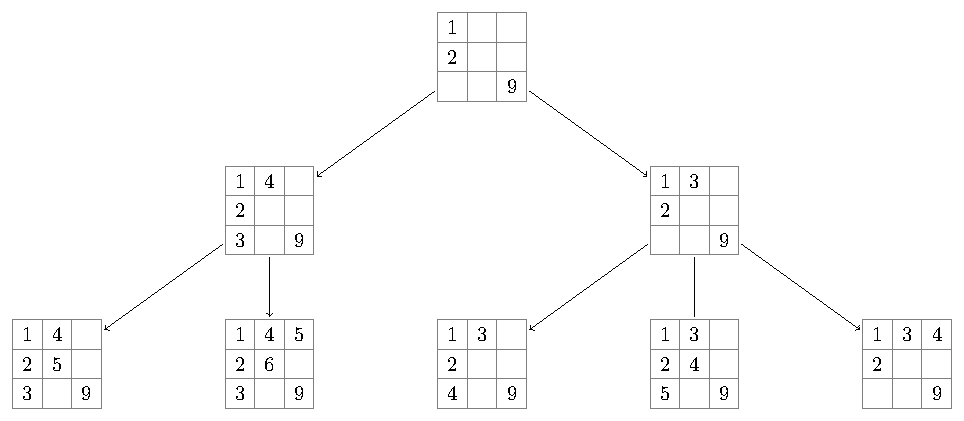
\includegraphics[width=\linewidth,page=1]{2021-08-07-figure-09}
\end{center}
Going down the branch on the left-hand side, we count $3$ cases on the left and $2$ cases on the right. Going down on the right-hand side, we count $5$ cases on the left, $6$ cases down the middle, and $5$ cases on the right, for a total of $3+2+5+6+5=21$. Since there were two possibilities for placing $2$ in the first square, the total number of cases is double $21$.
\begin{empheq}[box={\mathbox[colback=white]}]{equation*}
    42
\end{empheq} 
\end{answer}
%%%%%%%%%%%%%%%%%%%%%%%%%%%%%%%%%%%%%%%%%%%%%%%%%%%%%%%%%%%%%%%%%%%%%%%%

\iftoggle{showAnswers}{\newpage}

%%%%%%%%%%%%%%%%%%%%%%%%%%%%%%%%%%%%%%%%%%%%%%%%%%%%%%%%%%%%%%%%%%%%%%%%
\subsection*{10.}

\nopagebreak

A subset $B$ of the set of integers from 1 to 100, inclusive, has the property that no two elements of $B$ sum to 125. What is the maximum possible number of elements in $B$?

\fbox{(A) $50$ \quad (B) $51$ \quad (C) $62$ \quad (D) $65$ \quad (E) $68$}

\begin{answer}
Since the largest admissible integer is $100$, the integers from $1$ to $24$ cannot be paired to add up to $125$. Integers greater than $24$ can always be paired with an integer between $1$ and $100$, so we must exclude one of the numbers in the pair. Since there are $76$ such integers, we exclude half  of them, or $76/2=38$. The maximum possible number of elements is therefore $24+38=62$.

Which integer between $25$ and $100$ we choose to exclude has no incidence. For instance, consider the pair $(25, 100)$, which adds up to $125$. Whether we exclude $25$ or $100$, we get the same answer. 
\begin{empheq}[box={\mathbox[colback=white]}]{equation*}
    62
\end{empheq} 
\end{answer}
%%%%%%%%%%%%%%%%%%%%%%%%%%%%%%%%%%%%%%%%%%%%%%%%%%%%%%%%%%%%%%%%%%%%%%%%

\iftoggle{showAnswers}{\newpage}

\end{document}
